In this module you will learn
\begin{itemize}
	\item how to start modelling a physical phenomenon into a differential equation
\end{itemize}

\hfill \\


We started by studying some mathematical modelling in chapter 1. Then, we just used mathematical tools that we learned before. 

We now want to focus on mathematical models that arise from physical applications. These will often take the form of one or more differential equations.

The modelling of the situation will develop in a similar way.


\paragraph{\emph{Step 1.}} Defining the problem \\

As before, we should start by thinking about what our ultimate goal is. 
Once we settle on a goal, we define it as the function we want to study.

\begin{example}

\begin{minipage}{.7\textwidth}
In this module, we are going to think about the catapult problem from Module 9 - Slope Fields. \\

A catapult throws a projectile into the air.

Our goal is to track the height (in metres) of the projectile from the ground.

This means that we have a goal: to find the height of the projectile at every moment in time after it is launched.
\end{minipage}\hfill
\begin{minipage}{100pt}
	\includegraphics*[width=100pt]{images/module9-catapult.pdf}	
\end{minipage}
\hfill \\[10pt]

This means that we define
\begin{itemize}
	\item $y(t) = $ height of the projectile, in metres, $t$ seconds after it was launched from the catapult.
\end{itemize}

\end{example}

\hfill \\

\paragraph{\emph{Step 2.}} Building a mind map \\

A mind map will help us identify the notions that we want to include in our model.


\begin{example}

In the catapult example, since we decided to study the projectile's height, we need to find everything that affects its height.

\begin{center}
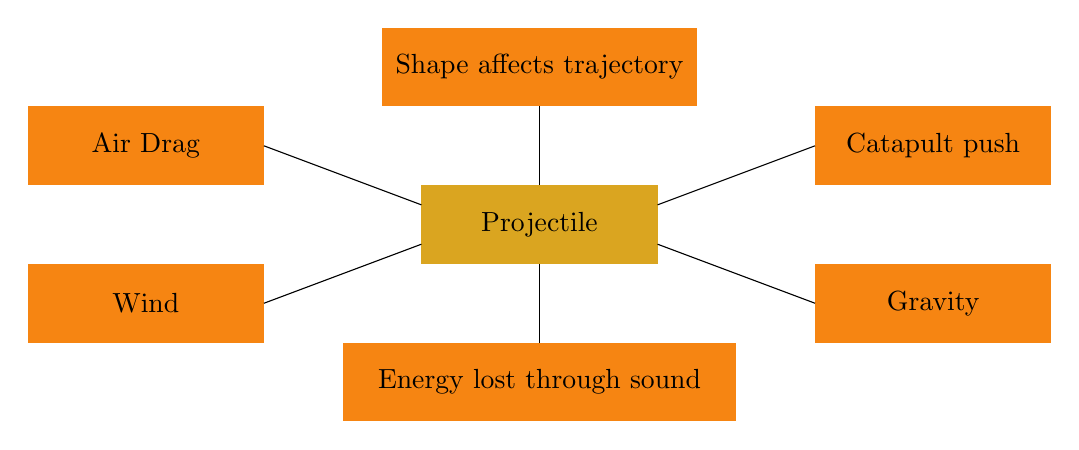
\begin{tikzpicture}
	\fill[color=Goldenrod] (0,0) rectangle (3,1) node[pos=.5] {\color{black}Projectile};
	\fill[color=BurntOrange] (5,1) rectangle (8,2) node[pos=.5] {\color{black}Catapult push};
	\fill[color=BurntOrange] (5,-1) rectangle (8,0) node[pos=.5] {\color{black}Gravity};
	\fill[color=BurntOrange] (-5,1) rectangle (-2,2) node[pos=.5] {\color{black}Air Drag};
	\fill[color=BurntOrange] (-5,-1) rectangle (-2,0) node[pos=.5] {\color{black}Wind};
	\fill[color=BurntOrange] (-1,-2) rectangle (4,-1) node[pos=.5] {\color{black}Energy lost through sound};
	\fill[color=BurntOrange] (-0.5,2) rectangle (3.5,3) node[pos=.5] {\color{black}Shape affects trajectory};
	\draw (3,0.75) -- (5,1.5);
	\draw (3,0.25) -- (5,-0.5);
	\draw (0,0.75) -- (-2,1.5);
	\draw (0,0.25) -- (-2,-0.5);
	\draw (1.5,0) -- (1.5,-1);
	\draw (1.5,1) -- (1.5,2);
\end{tikzpicture}
\end{center}

We can include more layers to these topics if we want.

\end{example}


\hfill \\

\paragraph{\emph{Step 3.}} Make assumptions \\

This is a fundamental step in any modelling endeavour. The real world is too complicated, so we make assumptions that simplify our model.

This has two main consequences:
\begin{enumerate}
	\item It makes our model simpler and easier to study;
	\item It creates constraints on our model: it is only valid under certain conditions.
\end{enumerate}

\begin{example}

Let us discuss the topics included in the mind map above:
\begin{itemize}
	\item Catapult Push -- the catapult pushes on the projectile for a small period of time when $t<0$. If we are considering only $t\geq 0$, then this will likely provide us with some starting conditions for the projectile
	\item Gravity -- The height of the projectile is affected by gravity. We have a choice to make:
	\begin{itemize}
		\item assume that the Earth is flat and gravity is constantly accelerating the projectile downwards;
		\item assume that the Earth is spherical and gravity is constantly accelerating the projectile towards the centre of the Earth;
		\item assume that the Earth is spherical and gravity is a force accelerating the projectile towards the centre of the Earth with a magnitude that decreases with the square of the distance to the centre of the Earth
		\item or other more complicated and more accurate models.
	\end{itemize}
	
	\item Air Drag -- air is making it hard for the projectile to move forward. We have another choice to make:
	\begin{itemize}
		\item assume that the air drag is a force that accelerates the projectile in the direction opposite to its movement and with magnitude proportional to its speed;
		\item assume that the air drag is a force that accelerates the projectile in the direction opposite to its movement and with magnitude proportional to the square of its speed;
		\item or other more complicated and more accurate models.
	\end{itemize}
\end{itemize}
	
I will leave it to you to think about the remaining three topics in the mind map. \\


We now need to make a decision about what to assume. \\

To keep this model simple, let us assume the following:
\begin{enumerate}
	\item The projectile's height will stay within a small range: $y(t) \in [0,100]$. Is this reasonable for a catapult?

		This means that we can consider the first of the gravitational models above: define gravitational acceleration as a constant $-g$.
		
	\item The projectile will not move very fast, so we can approximate the air drag to be directly proportional to the speed: define air drag acceleration as $\pm \gamma v$, where $\gamma>0$ is a constant that depends on the projectile and $v$ is the velocity of the projectile. Which sign should we have?

	\item Again, the projectile will not move very fast, so we can approximate the air drag to use only the vertical speed of the projectile: define air drag acceleration as $\pm \gamma v_y$, where $\gamma>0$ is a constant that depends on the projectile and $v_y$ is the vertical velocity of the projectile. Which sign should we have?

	\item The shape of the projectile will affect air drag in the form of the constant $\gamma>0$.

	\item Assume that for a medieval catapult (as in the drawing above), the other components are negligible.

\end{enumerate}

We come out of this step with some conditions for the validity of our model and some new constants and terms to use in our model.

\end{example}

\hfill \\

\paragraph{\emph{Step 4.}} Construct a model \\

This is the part where we put together the last three steps into one (or a system of) differential equations.

This should not be a difficult part if the last three steps were completed carefully.

\begin{example}

Summary of Steps 1--3:
\begin{itemize}
	\item \textbf{Goal:} study $y(t) = $ height of a projectile in metres, $t$ seconds after being released from a catapult
	\item \textbf{Forces:}
	\begin{itemize}
		\item Gravity: constant acceleration $-g$
		\item Air Drag: acceleration $\pm \gamma y'(t)$
	\end{itemize}
	\item \textbf{Conditions:}
	\begin{itemize}
		\item $y(t) \in [0,100]$
		\item Air drag should really by quadratic, but in this example we will consider this as an academic case.
	\end{itemize}
\end{itemize}

So the model we end up is:
$$
F_y = \substack{\text{vertical component}\\\text{of force}} = -g \pm \gamma y'.
$$

Now we bring a little bit of a Physics class into here: Newton's 2$^{\rm nd}$ Law states that \quad $F = m a$ \quad, so we obtain the model
$$m y''(t) =  -g \pm \gamma y'(t).$$
\end{example}



\paragraph{\emph{Step 5.}} Model Assessment

We just found a differential equation (model) for our situation. It is now time to test it to make sure that it behaves correctly.

For this step, we need to obtain a solution of the differential equation, either by solving it mathematically and finding a formula for the solution, or by approximating the solution numerically (see Module \ref{NumericalMethods}).

Then we need to check if the differential in one of several ways:
\begin{itemize}
	\item We can test it empirically: make an experiment and compare the results of the experiment with the results of the model
	\item We can test it mathematically: change the parameters and the initial conditions to make sure that we know how the model should behave and test some qualitative aspects of the model
\end{itemize}

\begin{important}
Even if the model passes all the tests, it might still not be correct.

Also, if it fails one test, it might mean that the model is incorrect, or that it has some limitations that are more subtle and we hadn't thought about them.	
\end{important}

\begin{example}
We have found the following model:
\begin{itemize}
	\item $y(t) = $ height of a projectile in metres, $t$ seconds after being released from a catapult
	\item It satisfies:
		$$m y''(t) =  -g + \gamma y'(t).$$
	(note that I chose the $+$ sign for the air drag component)

	\item Constraints:
	\begin{itemize}
		\item $y(t) \in [0,100]$;
		\item $\gamma >0$ is the drag constant: more air drag for larger values of $\gamma$;
	\end{itemize}
\end{itemize}	

This differential equation tells us what the second derivative, $y''(t)$, of $y(t)$ is given the first derivative $y'(t)$.
This means that to start solving the problem, we need to know what the initial values for $y'(t)$ and $y(t)$ are.

Need to know the starting conditions:
\begin{itemize}
	\item $y(t_0) = y_0$;
	\item $y'(t_0) = v_0$.
\end{itemize}

For this example, consider a situation where:
\begin{itemize}
	\item $g, \gamma >0$ can take any value.
	\item $y(0) = 0$;
	\item $y'(0) = g/\gamma > 0$;
\end{itemize}

The projectile is being catapulted from the ground with a positive velocity, so we expect it to go up for a while and then come back down to the ground.

What happens is 
$$
y''(0) = -g + \gamma y'(0) = 0,
$$
so the initial acceleration is 0, which means that the velocity is not changing.

The result is a function with constant velocity equal to its initial velocity:
\begin{itemize}
	\item $y(t) = \frac{g}{\gamma}t.$
\end{itemize}

This means that the height of the projectile keeps increasing, so the \emph{projectile never falls back to the ground}! \\

This means that there is a problem with our differential equation:
\begin{itemize}
	\item Is the model incorrect? 
	\item Is there a limitation on the initial velocity that we were not aware of?
\end{itemize}
\hfil

We must check our process again and correct it.
\end{example}




\paragraph{\emph{Step 6.}} Putting it all together in a report

We're not going to elaborate much on this step. For more on the subject, please check Module \ref{report}.





\begin{video}
\begin{itemize}
	\item \qrvideo{https://youtu.be/njg8xwMviGQ}
	\item \qrvideo{https://youtu.be/nKDsJB8iwb0}
\end{itemize}	
\end{video}

